% !TEX root = ../paper.tex

\section{Introduction}

Nonnegative Matrix Factorization (NMF) has been demonstrated to be an effective tool for unsupervised learning problems including clustering \cite{XLG03, SBPP06, DHS05}. 
An NMF consists of two tall-and-skinny non-negative matrices whose product approximates a nonnegative data matrix.
That is, given an $m\times n$ data matrix $\M{A}$, we seek nonnegative matrices $\M{W}$ and $\M{H}$ that each have $k$ columns so that $\M{A} \approx \M{W}\M{H}^\Tra$.
Each pair of corresponding columns of $\M{W}$ and $\M{H}$ form a latent component of the NMF.
If the rows of $\M{A}$ correspond to features and the columns to samples, the $i$th row of the $\M{H}$ matrix represents the loading of sample $i$ onto each latent component and provides a soft clustering.
Because the $\M{W}$ factor is also nonnegative, each column can typically be interpreted as a latent feature vector for each cluster.

Hierarchical clustering is the process of recursively breaking a group into two similar groups until every sample is a cluster by itself. That is., we consider all the data points as a single cluster and in each iteration, the data points in the current cluster are split into two separate clusters till there is only one sample in a cluster.
While standard NMF is interpreted as a flat clustering, it can also be extended for hierarchical clustering.
Kuang and Park \cite{KP13} propose a method that uses rank-2 NMF to recursively bipartition the samples.
An NMF with $k=2$ determines a row of $\M{H}$ of length 2 for each sample that determines its part membership.
By recursively bipartitioning the samples in each part, the method determines a binary tree such that each sample belongs to a unique leaf and internal nodes of the tree determine higher-level clusters of the samples.
A single latent feature vector for each node can also be used for interpreting clusters.
Similarly, Du et al. \cite{DKDP17} show that the latent features vectors of the leaves can also be used to initialize a $\M{W}$ within an algorithm for flat NMF, yielding fast convergence and overall speedup compared to initializing the algorithm with random data.
We discuss the hierarchical method in more detail in \Cref{sec:prelim} and \Cref{sec:seqalgs}.

We illustrate the output of the hierarchical clustering method with an example data set and output tree.
Following Gillis et al. \cite{GKP15}, we apply the method to a hyperspectral imaging (HSI) data set of the Washington, D.C~national mall, which has pixel dimensions $1280 \times 307$ and 191 spectral bands.
\Cref{fig:dc} visualizes the output tree with 6 leaves along with their hierarchical relationships.
The root node, labeled 0, is a flattening of the HSI data to a 2D grayscale image.
Each other node is represented by an overlay of the member pixels of the clusters (in blue) on the original grayscale image.
The first bipartitioning separates vegetation (cluster 1) from non-vegetation (cluster 2), the bipartitioning of cluster 1 separates grass (cluster 3) from trees (cluster 4), the bipartitioning of cluster 2 separates buildings (cluster 5) from sidewalks/water (cluster 6), and so on.
If the algorithm continues, it chooses to split the leaf node that provides the greatest benefit to the overall tree, which can be quantified as a node's ``score'' in various ways.
The algorithm proceeds to split nodes until a target number of leaves is obtained, until no node is worth splitting, or some other stopping criterion is met.

While the hierarchical clustering method offers advantages in terms of interpretation as well as execution time compared to flat NMF, implementations of the algorithm are limited to single workstations and the dataset must fit in the available memory.
Currently available implementations can utilize multiple cores via MATLAB \cite{KP13} or explicit shared-memory parallelization in the SmallK library \cite{SmallK}.

{\em The goal of this work is to use distributed-memory parallelism to scale the algorithm to large datasets that require the memory of multiple compute nodes and to high processor counts.}
While flat NMF algorithms have been scaled to HPC platforms \cite{FKPB15,BW09,MESPS20,KBP17}, our implementation is the first to our knowledge to scale a hierarchical NMF method to 1000s of cores. 
As discussed in detail in \Cref{sec:paralgs}, we choose to parallelize the computations associated with each node in the tree, which involve a Rank-2 NMF and the computation of the node's score.
We choose a data matrix distribution across processors that avoids any redistribution of the input matrix regardless of the data-dependent structure of the tree's splitting decisions so that the communication required involves only the small factor matrices.
Analysis of the algorithm shows the dependence of execution time on computation and communication costs as well as on $k$, the number of clusters computed.
In particular, we confirm that many of the dominant costs are logarithmic in $k$, which is favorable to the linear or sometimes superlinear dependence of flat NMF algorithms.

We demonstrate in \Cref{sec:results} the efficiency and scalability of our parallel algorithm on three data sets, including the HSI data of the DC mall and an image classification data set involving skin melanoma.
The experimental results show that our parallelization of Rank-2 NMF is highly scalable, maintaining computation bound performance on 1000s of cores.
We also show the limits of strong scalability when scaling to large numbers of clusters (leaf nodes), as the execution time shifts to becoming interprocessor bandwidth bound and eventually latency bound.
The image classification data set requires 800 GB of memory across multiple nodes to process, and in scaling from 10 nodes to 80 nodes of the Summit supercomputer (see \Cref{sec:summit}), we demonstrate parallel speedups of 7.1$\times$ for a single Rank-2 NMF and ZZ$\times$ for a complete hierarchical clustering.

\GB{we should have perhaps compared against SmallK and also against flat NMF...}

\begin{figure}
% !TEX root = ../paper.tex

\resizebox{\columnwidth}{!}{
\begin{tikzpicture}
    \node[inner sep=0pt] (original) at (0,0)
        {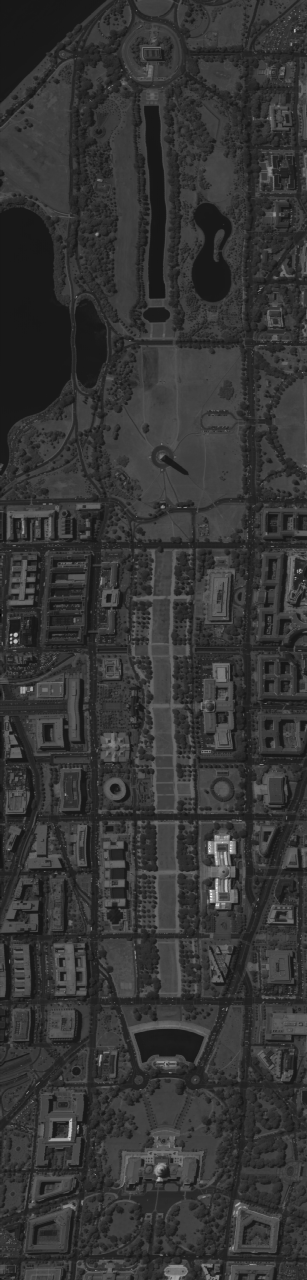
\includegraphics[width=0.8cm,height=3.2cm]{data/DC/0.png}};
        \draw[thick,->] (-0.4,0.8) .. controls (-3,0.8) .. (-3,-0.4);
        \node[inner sep=0pt] (1) at (-3,-2)
            {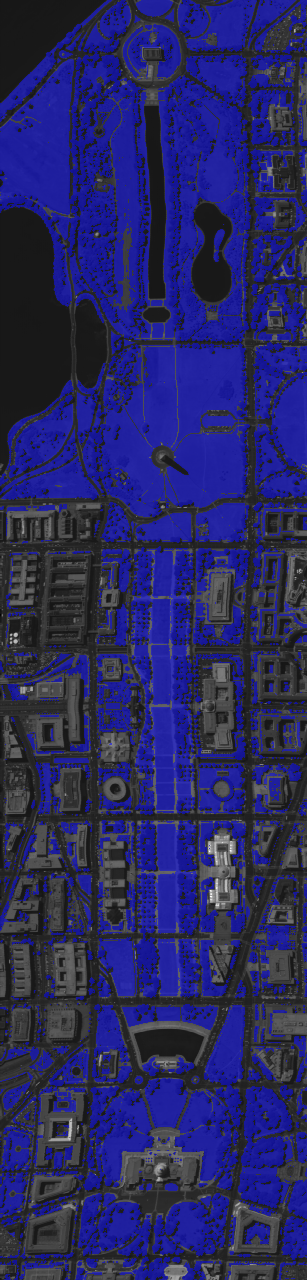
\includegraphics[width=0.8cm,height=3.2cm]{data/DC/1.png}};
            \draw[thick,->] (-2.6,-1.2) .. controls (-1.6,-1.2) .. (-1.6,-2.4);
            \node[inner sep=0pt] (3) at (-1.6,-4)
                {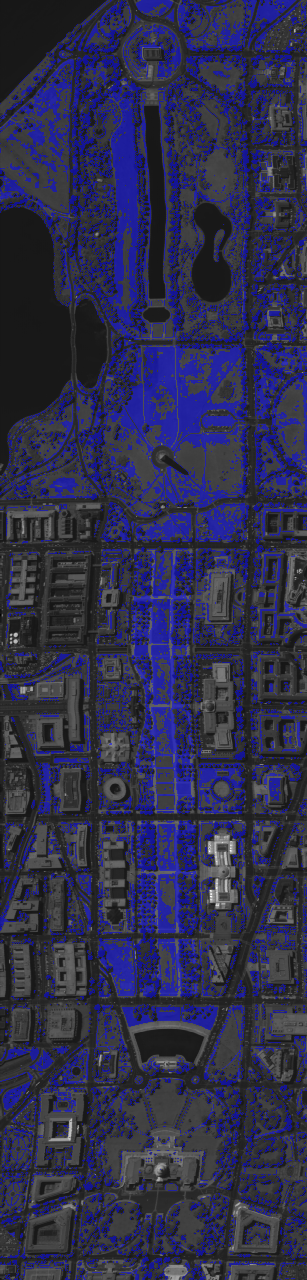
\includegraphics[width=0.8cm,height=3.2cm]{data/DC/3.png}};
                \draw[thick,->] (-2,-3.2) .. controls (-2.5,-3.2) .. (-2.5,-4.4);
                \node[inner sep=0pt] (7) at (-2.5,-6)
                    {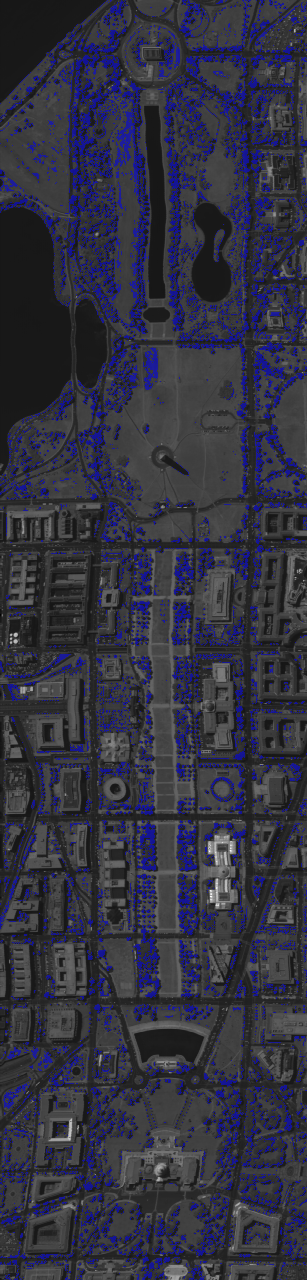
\includegraphics[width=0.8cm,height=3.2cm]{data/DC/7.png}};
                \draw[thick,->] (-1.2,-3.2) .. controls (-0.7,-3.2) .. (-0.7,-4.4);
                \node[inner sep=0pt] (8) at (-0.7,-6)
                    {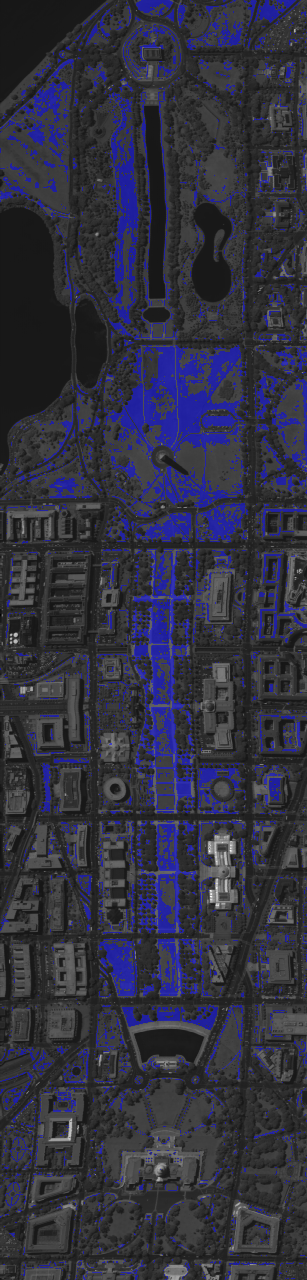
\includegraphics[width=0.8cm,height=3.2cm]{data/DC/8.png}};
            \draw[thick,->] (-3.4,-1.2) .. controls (-4.4,-1.2) .. (-4.4,-2.4);
            \node[inner sep=0pt] (4) at (-4.4,-4)
                {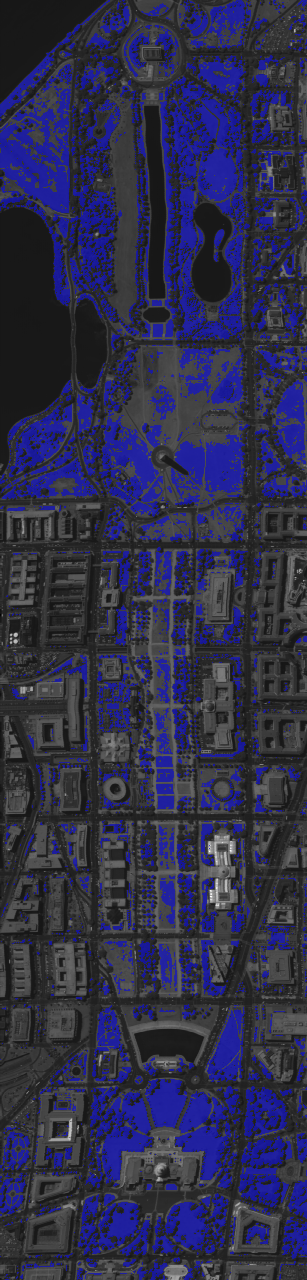
\includegraphics[width=0.8cm,height=3.2cm]{data/DC/4.png}};
        \draw[thick,->] (0.4,0.8) .. controls (3,0.8) .. (3,-0.4);
        \node[inner sep=0pt] (2) at (3,-2)
            {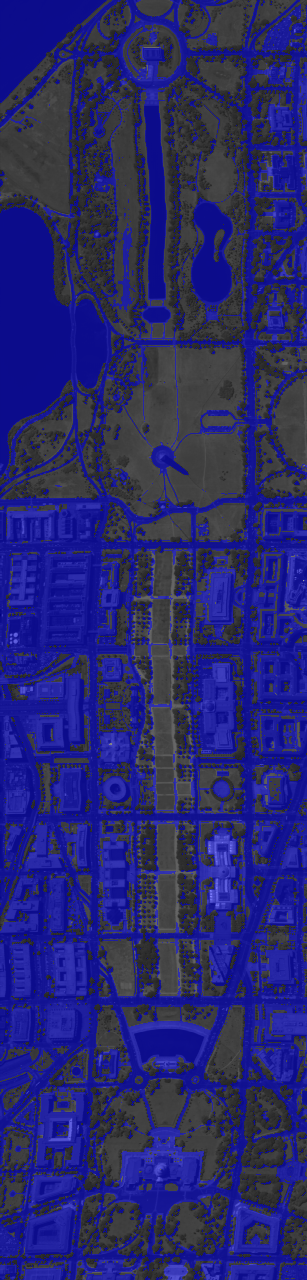
\includegraphics[width=0.8cm,height=3.2cm]{data/DC/2.png}};
            \draw[thick,->] (3.4,-1.2) .. controls (4.4,-1.2) .. (4.4,-2.4);
            \node[inner sep=0pt] (5) at (4.4,-4)
                {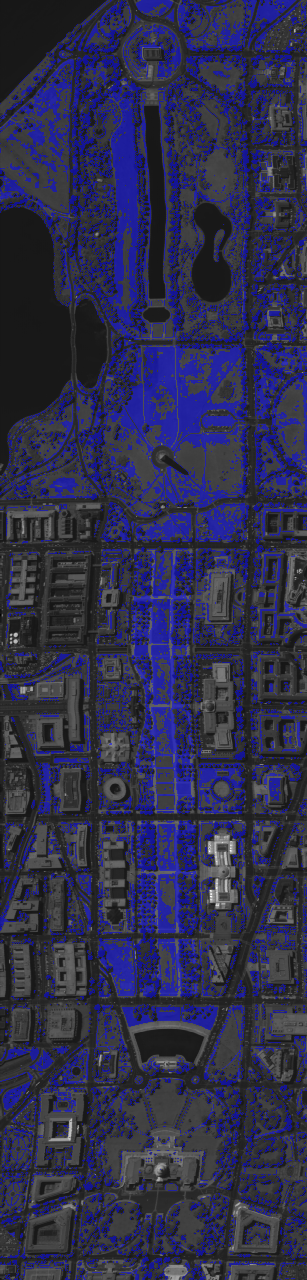
\includegraphics[width=0.8cm,height=3.2cm]{data/DC/3.png}};
            \draw[thick,->] (2.6,-1.2) .. controls (1.6,-1.2) .. (1.6,-2.4);
            \node[inner sep=0pt] (6) at (1.6,-4)
                {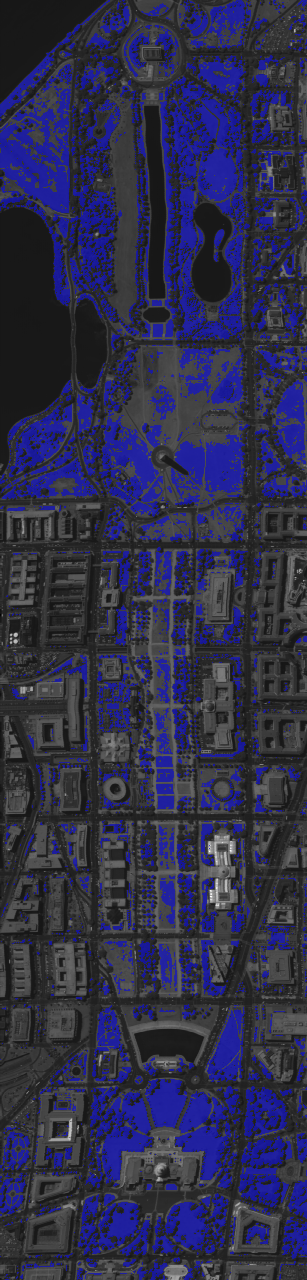
\includegraphics[width=0.8cm,height=3.2cm]{data/DC/4.png}};
                \draw[thick,->] (1.2,-3.2) .. controls (0.7,-3.2) .. (0.7,-4.4);
                \node[inner sep=0pt] (13) at (0.7,-6)
                    {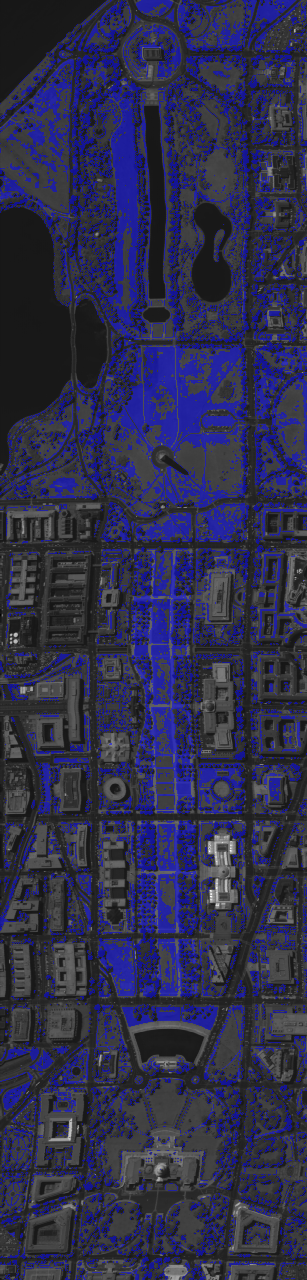
\includegraphics[width=0.8cm,height=3.2cm]{data/DC/3.png}};
                    \draw[thick,->] (2,-3.2) .. controls (2.5,-3.2) .. (2.5,-4.4);
                \node[inner sep=0pt] (14) at (2.5,-6)
                    {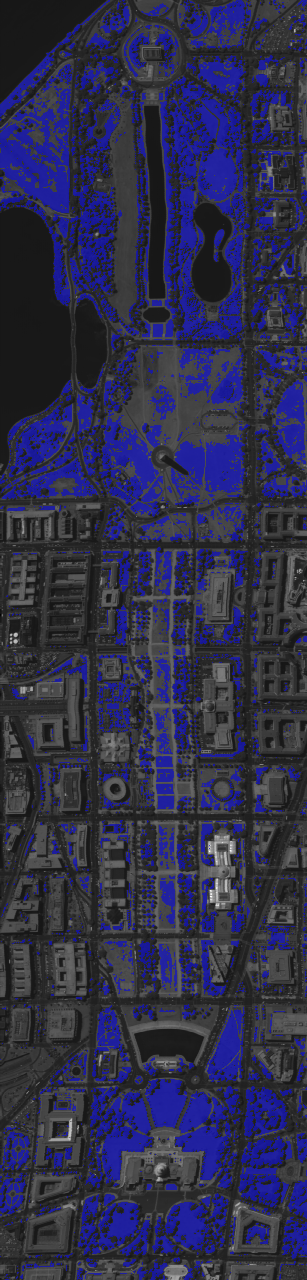
\includegraphics[width=0.8cm,height=3.2cm]{data/DC/4.png}};
\end{tikzpicture}
}
\caption{Hierarchical Clustering of DC Mall Hyperspectral Image}
\label{fig:dc}
\end{figure}
